\section{Шумоподавление}

\subsection{Постановка задачи}

Шумоподавление -- процесс выделения полезного сигнала из наложения
полезного сигнала и шума.

Предположим, что требуется записать речь человека на улице.
В таких условия помимо голоса человека на запись может попасть
шум дорожного движения,
фоновая речь людей,
шум встречных воздушных потоков 
и прочие звуки окружающего пространства.

В данном случае задача шумоподавления состоит в том, чтобы выделить
речь человека среди шума улицы. 

Шум в звуковом сигнале определяется как беспорядочные колебания
звуковых волн.

Формально взаимодействие полезного (целевого) сигнала и шума
описывается следующей формулой:

\begin{equation*}
    \textstyle y_t = s_t + n_t, 
\end{equation*}

\begin{explanation}
    %\item[где]  $t$    - рассматриваемый промежуток времени;
    \item[где]  $s_t$   - полезный сигнал;
    \item       $n_t$   - шум;
    \item       $y_t$   - сигнал из реальной записи.
\end{explanation}

Формализация задачи шумоподавления имеет следующий вид:
имея зашумленный сигнал $y_t$, 
необходимо найти значение $\hat{y_t}$, 
максимально близкое к исходному сигналу $s_t$.

\subsection{Классификация шумов}

Шум, как и любой другой звуковой сигнал, 
имеет свою природу и уникальные, присущие
ему признаки.

Существует множество различных классификаций шумов, основыми из которых
являются следующие:

\begin{itemize}
    \item по спектру;
    \item по характеру спектра;
    \item по происхождению;
    \item по частоте;
    \item по временным характеристикам.
\end{itemize}

Однако, если стоит задача удалить шумы в записи речи,
в первую очередь следует учитывать категоризацию шумов
по их временным характеристикам \cite{asr_end2end}.

На рисунке \ref{fig:section4:time_classification} представлена 
классификация шумов на основе их временных характеристик.

\begin{figure}[h!]
    \centering
    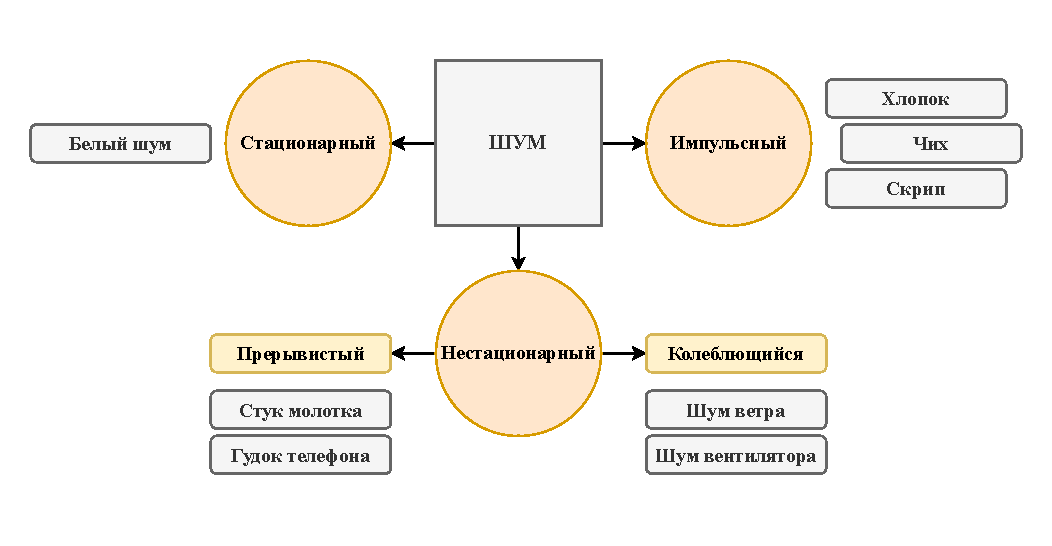
\includegraphics[scale=0.8]{S4IM1.pdf}
    \caption{Классификация шумов по временным характеристикам}
    \label{fig:section4:time_classification}
\end{figure}

Стационарные и колеблющиеся шумы, как правило, образованы
постоянными процессами, в то время как
прерывистые и импульсные -- резкими единоразовыми.
Прерывистый шум можно представлять как повторяющийся с некоторой
периодичностью импульсный шум.

Категории шума определены для того, чтобы разграничивать шумы по
сложности их подавления. 
Основная сложность задачи шумоподавления заключается в 
непредсказуемости шумов, которые могут возникнуть в звуковом сигнале. 

Достаточно легко избавиться от стационарного шума, потому что
легко определить его порог громкости в спектре исходного сигнала,
так как шум будет равномерно распределен по всему звуковому сигналу,
и в фрагментах тишины основной составляющей будет его амплитуда.

Процесс подавления колеблющихся и прерывистых шумов более сложен,
посколько трудно определить точное расположение таких шумов в
исходном звуковом сигнале.

Наиболее сложной является задача подавления импульсных шумов, так как 
ввиду непредсказуемости определение их местоположения 
в звуковом сигнале затруднительно.

На рисунке \ref{fig:section4:noise_pyramid} изображена 
пирамида сложности подавления шума в зависимости от его сложности:

\begin{figure}[h!]
    \centering
    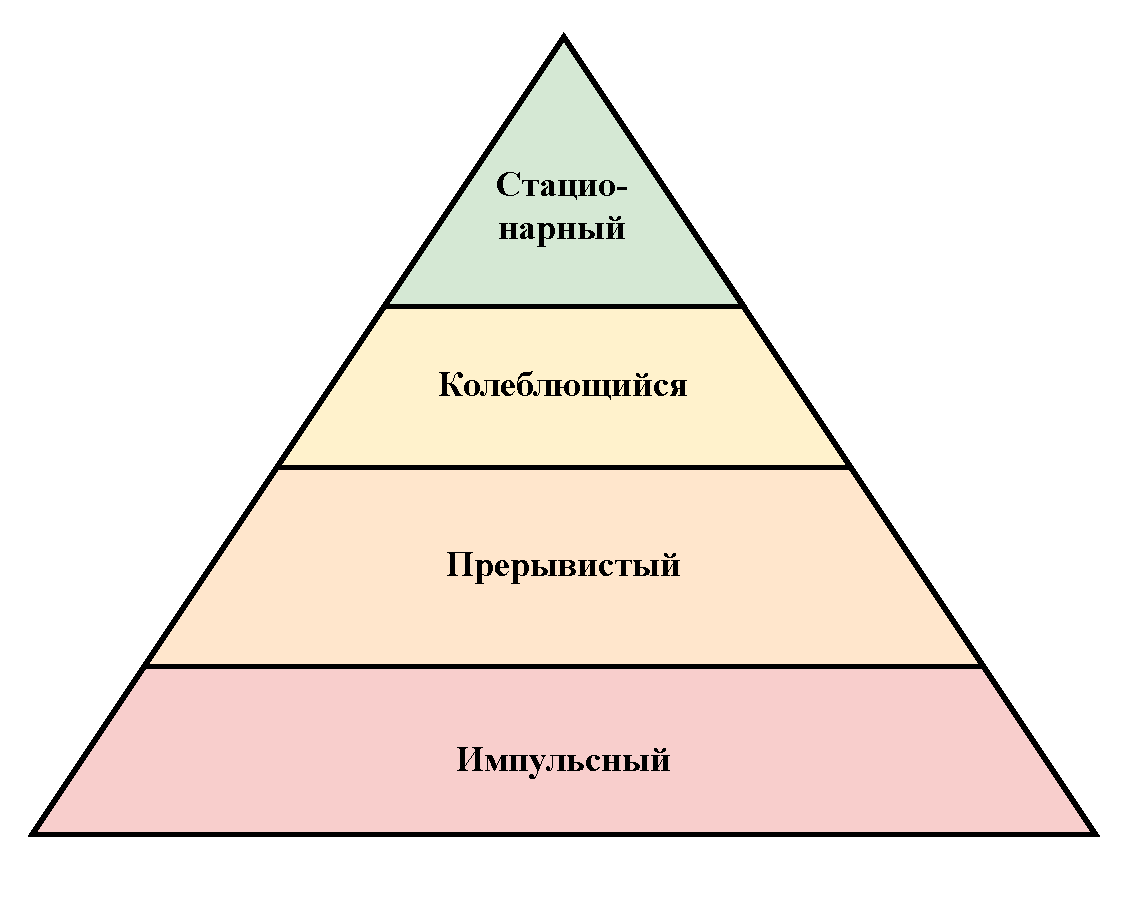
\includegraphics[scale=0.6]{S4IM2.pdf}
    \caption{Пирамида сложности шумоподавления}
    \label{fig:section4:noise_pyramid}
\end{figure}

Если задачи наверху пирамиды можно решить классическими методами,
то задачи шумоподавления из нижней части пирамиды можно решить
только методами машинного обучения. Кроме того, нейросетевой
подход позволяет решить задачу шумоподавления для всех типов,
в то время как вычислительные методы решают задачи подавления
определенного типа шумов.

\subsection{Используемые методы машинного обучения}

Наиболее эффективным методом машинного обучения в шумоподавлении
и улучшении речевого сигнала является
использование сверточных нейронных сетей.

Общий принцип нейросетевых архитектур обработки звука и речи:
наличие сверточного энкодера и декодера, выполняющих определение
источников шумов и их восстановления с последующим вычитанием
из исходного сигнала.

Среди архитектур сверточных нейронных сетей, 
используемых в шумоподавлении, можно выделить
WaveNet \cite{wavenet}, Tas-Net \cite{tasnet}, а также её модификацию Conv-Tas-Net. 

\subsection{Применение}

Методы шумоподавления используются при очистке аудио от лишних
звуковых сигналов для повторного воспроизведения.

Более сложной задачей является мгновенное шумоподавление -- 
шумоподавление и воспроизведение одновременно с записью речи.
Чаще всего такое шумоподавление используется для аудиоконференций в
Zoom, Discord, Skype, а также в таких мессенджерах как Telegram и VK. 

Как правило, при решении задачи мгновенного шумоподавления,
используются классические вычислительные методы, но помимо них
применяются и методы машинного обучения для очистки сигнала на лету.
Так, компания Microsoft по результатам соревнований DNS-Challenge
использовала наилучшие решения в областирекуррентных и сверточных сетей 
и адаптировала их под свою продукцию Skype и Teams \cite{skype}.

\begin{figure}[h!]
    \centering
    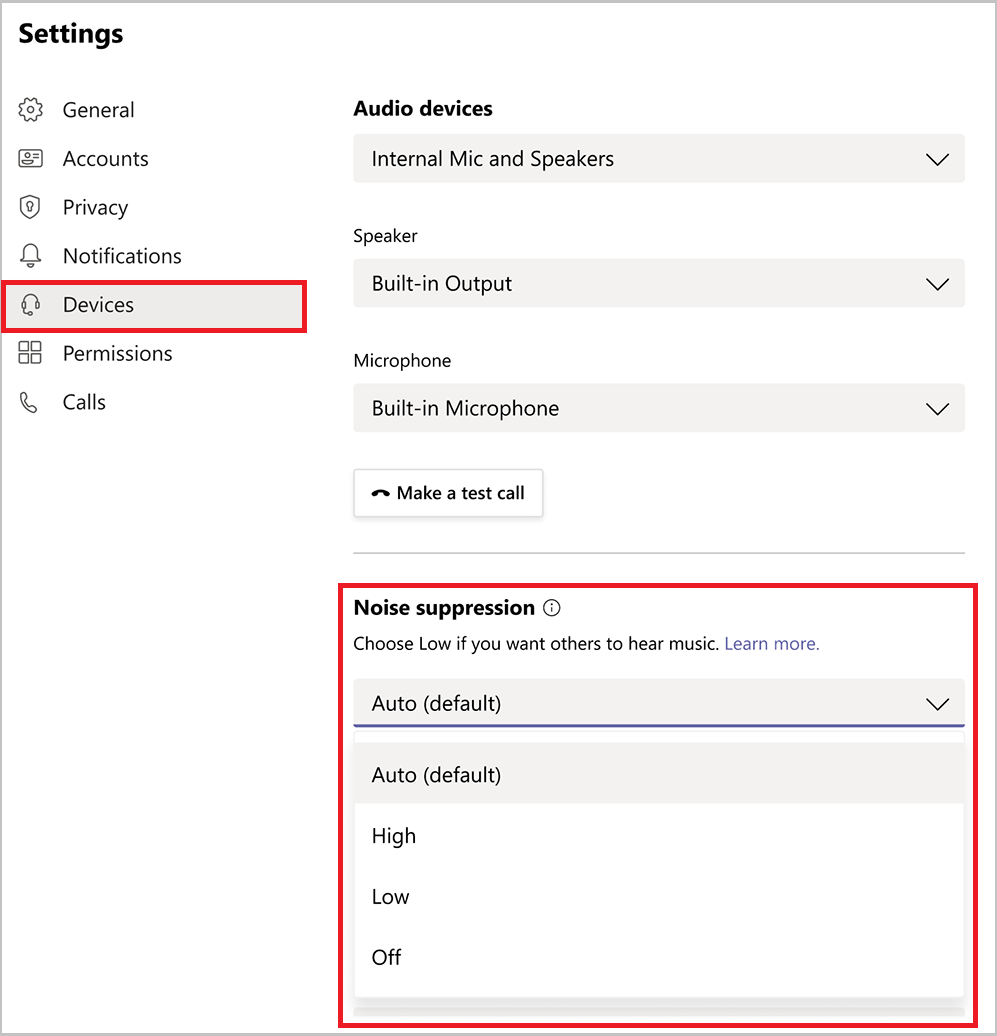
\includegraphics[scale=0.6]{S4IM3.png}
    \caption{Функция активного шумоподавления в Microsoft Teams}
\end{figure}